\chapter{PREVIOUS WORK} \label{sec:prevwork}

\section{Real-Time Versus Offline Rendering Techniques}
\paragraph{}
Rendering techniques can be broken down into two distinct categories: real-time and offline.  Offline rendering techniques require anywhere from seconds to many hours to render a single image.  Current offline rendering techniques are able to render ultra-realistic images that take into account many light sources as well as many types of lighting principles such as reflection, refraction, sub-surface light scattering, and others in very complex scenes consisting of millions of triangles and at high resolutions.  Real-time rendering techniques render images at a fast enough rate to support multiple frames a second and vary greatly in approach.  These techniques can be broken down into dynamic and static.  Dynamic scenes allow a user to interact with the scene by actively moving the geometry, the camera, or the light source whereas static scenes do not.  As opposed to offline techniques, real-time techniques have to make sacrifices and therefore can't be as scientifically accurate as offline techniques.  The goal of this paper is to create a real-time technique that supports a fully dynamic scene.  Regardless of whether the technique is offline or real-time, the algorithm used can trace it's roots back to a single equation, \textit{The Rendering Equation}.

\section{The Rendering Equation} \label{sec:render}
\paragraph{}
When discussing light transport in computer graphics, the most significant paper is \textit{The Rendering Equation} by Kajiya (1986).  In it, Kajiya presents an equation that generalizes most rendering algorithms.  Such a statement can be confirmed by the fact that all rendering equations try to recreate the scattering of light off of different types of surfaces and materials.  The rendering equation is an integral that is adapted from the study of radiative heat transfer for use in computer graphics with an aim at balancing the energy flow between surfaces.  The equation, however, is still an approximation because it does not take into account diffraction and it assumes that the space between objects, such as air, is of homogeneous refractive index meaning that light won't refract due to the particles in the air.

\begin{equation}
I(x,x') = g(x,x')[\epsilon(x,x')+\int_{S} \rho(x,x',x'')I(x',x'')dx''] \label{eqn:render}
\end{equation}

\paragraph{}
The rendering equation is broken down into 4 parts.  First, $I(x,x')$ is the intensity of light or energy of radiation passing from point $x'$ to point $x$ measured in energy of radiation per unit time per unit area.  Second, the geometry term, $g(x,x')$, indicates the occlusion of objects by other objects.  This term is either $0$, if $x$ and $x'$ are not visible from one another, or $1/r^2$ where $r$ is the distance between $x$ and $x'$ if $x$ and $x'$ are visible from one another.  Third, the emittance term, $\epsilon(x,x')$, measures the energy emitted from point $x'$ that reaches point $x$.  Lastly, the scattering term, $\rho(x,x',x'')$, is the intensity of energy scattered by a surface point $x'$ that originated from point $x''$ and then ends at point $x$.  As mentioned in the previous section, global illumination can be calculated using the Neumann series.  A Neumann series is a mathematical series of the form:
\begin{equation}
\sum_{k=0}^{\infty}T^k \label{eqn:neumann}
\end{equation}

where $T$ is an operator and therefore $T^k$ is a notation for $k$ consecutive operations of operator $T$. 

\paragraph{}
Furthermore, the rendering equation can also be approximated using the Neumann series.  This is done by rewriting the rendering equation above (\ref{eqn:render}) as:
\begin{equation}
I = g\epsilon +gMI \label{eqn:render2}
\end{equation}
where $M$ is the linear operator given by the integral in the rendering equation.  Next, we rewrite equation \ref{eqn:render2} as:
\begin{equation}
(1-gM)I = g\epsilon \label{eqn:render3}
\end{equation}
so that we can invert it to get:
\begin{equation}
I = g\epsilon + gMg\epsilon + gMgMg\epsilon +g(Mg)^3\epsilon + ... \label{eqn:render4}
\end{equation}
Equation \ref{eqn:render4} is a Neumann series of the form:
\begin{equation}
I = g\epsilon\sum_{k=0}^{\infty}(Mg)^k \label{eqn:render5}
\end{equation}
Equation \ref{eqn:render5} indicates that the rendering equation (equation \ref{eqn:render}) is the final intensity of radiation transfer as a sum of a direct term, a once scattered term, a twice scattered term, and so on.  Therefore, as mentioned in the previous chapter, indirect illumination can be calculated by summing the light incident on a surface due to the reflection of light $n$-times as $n$ approaches infinity.  The more scattered terms we include in the calculation, the better the approximation will be but with worse performance.  Therefore, in real-time applications, this needs to be avoided.  

\paragraph{}
Next, we show how the rendering equation can be seen has a generalization of most rendering algorithms, but first we must cover some other rendering techniques beginning with offline rendering techniques.

\section{Offline Rendering Techniques}
\paragraph{}
Key examples of offline rendering techniques are ray tracing, radiosity, and photon maps.  We begin with ray tracing.

\subsection{Ray Tracing}

\begin{figure}[h!]
  \centering
    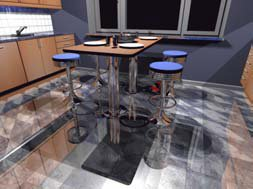
\includegraphics[width=0.5\textwidth]{raytraceSample.jpg}
  \caption{Image produced using ray tracing.}
	\label{fig:raytraceSample}
\end{figure}

\paragraph{}
Ray tracing is a technique for rendering an image of a three-dimensional scene by casting rays from a camera positioned somewhere in the scene.  Each ray is shot into the scene and it registers the first surface it hits.  From this surface point, additional rays go to each of the light sources to determine visibility to render shadows as well as to other surfaces to render reflections as shown in figure \ref{fig:raytraceCalc} from Ward, Rubinstein, and Clear (1988).  These rays can also be used to calculate other lighting phenomena such as refractions.

\begin{figure}[h!]
  \centering
    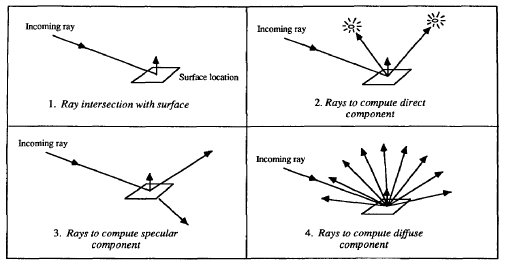
\includegraphics[width=1.0\textwidth]{raytraceCalc.jpg}
  \caption{Steps of ray tracing.}
	\label{fig:raytraceCalc}
\end{figure}

\paragraph{}
The rays from the camera can be cast into the scene using different sampling patterns and techniques such as one ray per pixel or many rays per pixel.  Also, the rays can be cast through the center of each pixel or through the use of stochastic sampling can be cast through non-uniformly spaced locations in each pixel to avoid aliasing artifacts or jaggies as shown in figures \ref{fig:sampling} and \ref{fig:jaggies} from Reeves, Salesin, and Cook (1987).

\begin{figure}[h!]
  \centering
    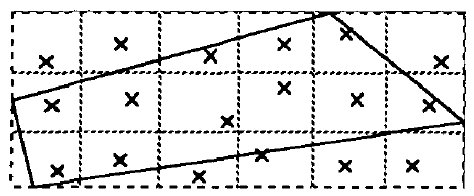
\includegraphics[width=0.5\textwidth]{sampling.jpg}
  \caption{Sampling non-uniformly spaced locations in each pixel.}
	\label{fig:sampling}
\end{figure}

\begin{figure}[h!]
  \centering
    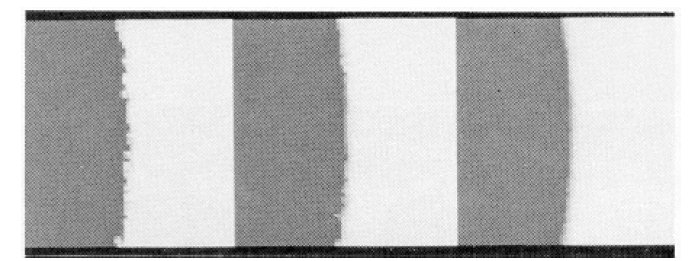
\includegraphics[width=0.5\textwidth]{jaggies.jpg}
  \caption{Image of aliasing artifacts known as jaggies. Better sampling results in softer edges.}
	\label{fig:jaggies}
\end{figure}

\paragraph{}
Ray tracing is able to recreate ultra-realistic scenes such as figure \ref{fig:raytraceSample} from Wald, Benthin, and Slusallek (2003) but at a high cost.  Examples of ray tracing techniques can be seen in the work of Whitted (1980), Cook (1986), and Ward et al. (1988).  With adaptations to ray tracing techniques and advances in technology, there now exist some interactive ray-tracing techniques mentioned in section \ref{sec:RT}.

\paragraph{}
Ray tracing can also be related to the rendering equation.  Whitted (1980) describes a new approximation for ray tracing by rewriting the Phong illumination model in order to improve the quality of specular reflections.  The Phong illumination model is a way of calculating lighting on a surface through the combination of three components: ambient, diffuse, and specular.  Diffuse is the reflection of light from rough surfaces, specular is the reflection of light on shiny surfaces, and the ambient component accounts for the amount of light that is scattered throughout the scene.  The ambient term is most similar to indirect lighting, but is a user-specified constant amount distributed uniformly throughout the scene to avoid any actual calculations.  The improved model from Whitted (1980) is written:
\begin{equation}
I = I_{a} + k_{d}\sum_{j=1}^{j=ls}(\bar{N}\cdot\bar{L}_{j})+k_{s}S + k_{t}T \label{eqn:raytrace1}
\end{equation}

where $S$ is the intensity of light incident from the specular reflection direction, $k_{t}$ is the transmission coefficient, and $T$ is the intensity of light from the transmitted light direction. $k_{s}$ and $k_{t}$ are coefficients that are to be used to try to accurately model the Fresnel reflection law, which is an equation that describes how light behaves when moving from one medium to another with a different refractive index.  Equation \ref{eqn:raytrace1} is in the form of equation \ref{eqn:render4} from Kajiya (1986) with $M$ as the sum of the reflection and refraction terms as well as the diffuse component. Then the term $g$ considers shadows and the ambient term can be approximated by the $\epsilon$ term.  Lastly, $M$ is approximated by summing over all the light sources rather than using integration.

\subsection{Radiosity}

\begin{figure}[h!]
  \centering
    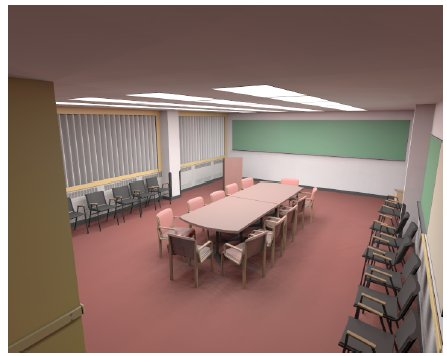
\includegraphics[width=0.5\textwidth]{radiositySample.jpg}
  \caption{Image rendered using radiosity.}
	\label{fig:radiositySample}
\end{figure}

\paragraph{}
Radiosity is a type of rendering technique that was adapted for use in computer graphics from the thermal engineering field.  The method is based on the fundamental Law of Conservation of Energy within a closed area.  This law states that energy can neither be created nor destroyed and that the energy in this closed area is to remain constant over time.  It provides a global solution for the intensity of light incident on each surface by solving a system of linear equations that describes the transfer of energy between each surface in the scene.  Examples of radiosity can be found in the works of Immel, Cohen, and Greenberg (1986) and Goral, Torrance, Greenberg, and Battalie (1984) and shown in figure \ref{fig:radiositySample} from Keller (1997).

\paragraph{}
Radiosity is a natural extension from the rendering equation (equation \ref{eqn:render}) since its focus is on balancing the flow of energy.  The only difference is that radiosity makes assumptions about the reflectance characteristics of the surface material.  The radiosity in the scene is found by taking the hemispherical integral of the energy leaving the surface called flux seen in figure \ref{fig:radiosityCalc1} from Immel et al. (1986).  This can be found using the following equation from Goral et al. (1984):
\begin{equation}
B_{j} = E_{j} + \rho_{j}H_{j} \label{eqn:radiosity1}
\end{equation}

where $B_{j}$ is the rate of energy leaving the surface $j$ measured in energy per unit time per unit area, $E_{j}$ is the rate of direct energy emission,  $\rho_{j}$ is the reflectivity of surface $j$, and $H_{j}$ is the incident radiant energy arriving at surface $j$ per unit time per unit area as depicted in figure \ref{fig:radiosityCalc2} from Goral et al. (1984).

\begin{figure}[h!]
  \centering
    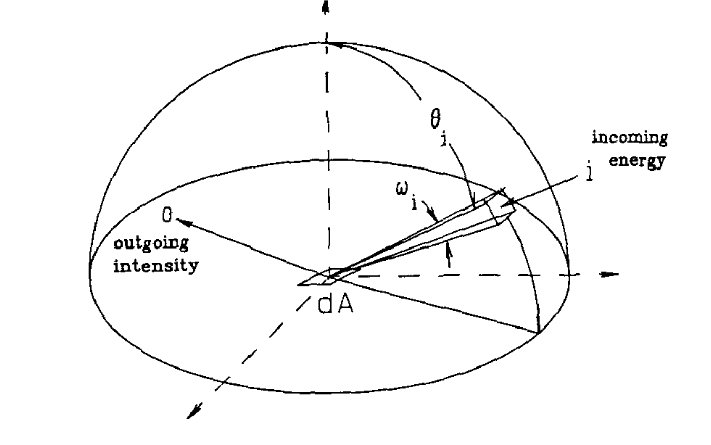
\includegraphics[width=0.75\textwidth]{radiosityCalc1.jpg}
  \caption{Hemispherical integral of the energy leaving the surface.}
	\label{fig:radiosityCalc1}
\end{figure}

\begin{figure}[h!]
  \centering
    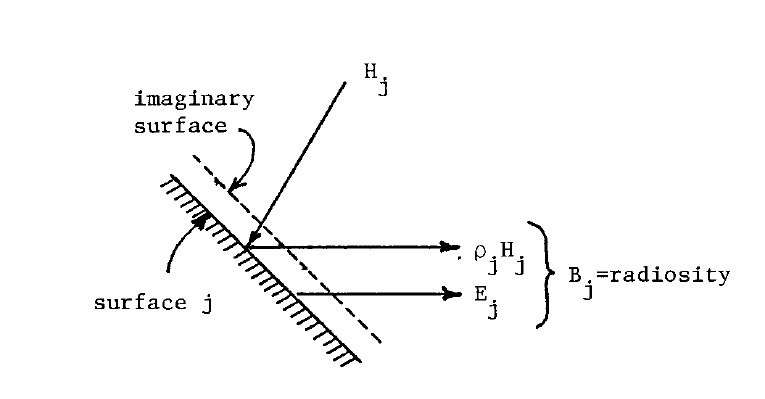
\includegraphics[width=0.75\textwidth]{radiosityCalc2.jpg}
  \caption{Illustration of equation \ref{eqn:radiosity1}.}
	\label{fig:radiosityCalc2}
\end{figure}

\paragraph{}
Equation \ref{eqn:radiosity1} can be derived using our rendering equation (equation \ref{eqn:render}) by Kajiya (1986) by integrating over all surfaces in the scene to calculate the hemispherical quantities, calculating the contribution of the emittance and reflectance terms by checking for occlusions, and by using those calculations the rendering equation becomes:
\begin{equation}
dB(x') = \pi[\epsilon_{0} + \rho_{0}H(x')]dx' \label{eqn:radiosity2}
\end{equation}

where $\epsilon_{0}$ is the hemispherical emittance of the surface element $dx'$, $\rho_{0}$ comes from the reflectance term, and $H$ is the hemispherical incident energy per unit time per unit area.  This adaptation of the rendering equation (equation \ref{eqn:radiosity2}) is the same as the radiosity equation shown above (equation \ref{eqn:radiosity1}).

\subsection{Photon Maps}

\begin{figure}[h!]
  \centering
    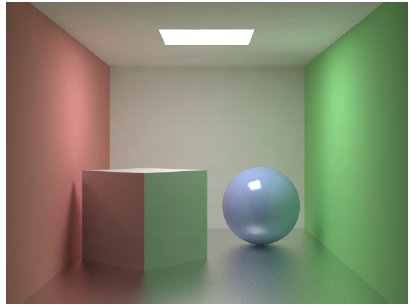
\includegraphics[width=0.5\textwidth]{photonSample.jpg}
  \caption{Image rendered using photon maps.}
	\label{fig:photonSample}
\end{figure}

\paragraph{}
Photon maps originally introduced by Jensen (1996) is a two pass global illumination method that produces images such as that seen in figure \ref{fig:photonSample}.  As mentioned in the Background section, Einstein coined the term photon for the particles present in the energy of light waves.  In the method of photon mapping, the term photon is used in a similar context.  The first pass of the method consists of making two photon maps by emitting packets of energy called photons from the light sources and storing where they hit surfaces in the scene as seen in figure \ref{fig:photonCalc}.  The second pass of the method calls for the use of a distribution ray tracer that is optimized using the data gathered in the photon maps.  Photon maps are able to render complex lighting principles such as the caustics seen in figure \ref{fig:photonCaustics}.

\begin{figure}[h!]
  \centering
    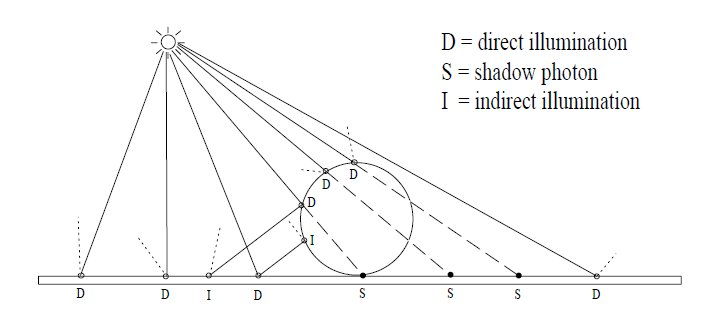
\includegraphics[width=1.0\textwidth]{photonCalc.jpg}
  \caption{Process of casting photons into the scene.}
	\label{fig:photonCalc}
\end{figure}

\begin{figure}[h!]
  \centering
    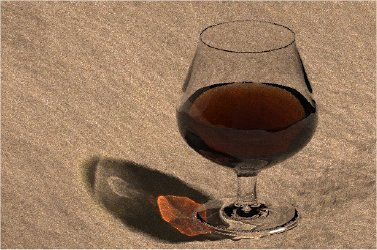
\includegraphics[width=0.5\textwidth]{photonCaustics.jpg}
  \caption{Example of caustics.}
	\label{fig:photonCaustics}
\end{figure}

\paragraph{}
Photon maps are an extension to the rendering equation (equation \ref{eqn:render}) as well.  During the second pass of the method, the scene is rendered by calculating the radiance by tracing a ray from the eye through the pixel and into the scene using ray tracing, and the radiance is computed at the first surface that the ray hits.  The surface radiance leaving the point of intersection $x$ in some direction is computed using this equation from Jensen (1996):
\begin{equation}
L_{s}(x,\psi_{r} = L_{e}(x,\psi_{r} + \int_{\Omega}(f_{r}(x,\psi_{i};\psi_{r})L_{i}(x,\psi_{i})\cos(\theta_{i})d\omega_{i}) \label{eqn:photon1}
\end{equation}

where $L_{e}$ is the radiance emitted by the surface, $L_{i}$ is the incoming radiance in the direction $\psi_{i}$, and $f_{r}$ is the BRDF or bidirectional reflectance distribution function, which is a four-dimensional function that describes how light is reflected at a surface point.  Lastly, $\Omega$ is the sphere of incoming directions.  This can be broken down into a sum of four components:
\begin{align}
  &\begin{aligned} \label{eqn:photon2}
    L_{r} &=  \int_{\Omega} (f_{r}L_{i,l}\cos(\theta_{i})d\omega_{i}) + \int_{\Omega}(f_{r,s}(L_{i,c}+L_{i,d})\cos(\theta_{i})d\omega_{i})\\
      &\qquad + \int_{\Omega} (f_{r,d}L_{i,c}\cos(\theta_{i})d\omega_{i}) +  \int_{\Omega}(f_{r,d}L_{i,d}\cos(\theta_{i})d\omega_{i}
  \end{aligned}
\end{align}

where the first term of equation \ref{eqn:photon2} is the contribution by direct illumination, the second term is the contribution by specular reflection, the third term is the contribution by caustics, and the fourth term is the contribution by soft indirect illumination.  Both equations \ref{eqn:photon1} and \ref{eqn:photon2} are direct adaptations from the rendering equation in as introduced by Kajiya (1986) (equation \ref{eqn:render}).

\subsection{Other Offline Rendering Techniques} \label{sec:otheroffline}
\paragraph{}
Many recent offline techniques have been influenced by real-time techniques most notably the idea of using virtual point lights or VPL's as introduced in \textit{Instant Radiosity} by Keller (1997).  This technique will be discussed in detail in the real-time rendering techniques section, but the main idea is that we can render indirect light through the use of a set of VPL's where we accumulate the contributions of each of these lights in multiple rendering passes.  This technique is used for rendering illumination from area lights, high dynamic range (HDR) environment maps or sun/sky models, single/multiple subsurface light scattering in participating media, and most importantly for our purposes indirect illumination.  For offline purposes, techniques typically call for the use of millions of VPL's to achieve higher quality renderings, however, many techniques attempt to mitigate the cost of using such a large number of lights.

\underline{Virtual Point Lights}: In \textit{Lightcuts: A Scalable Approach to Illumination} by Walter et al. (2005), it is discussed that when using many lights, as in the VPL method, the cost to render the scene scales linearly with the number of lights used.  This limits the number of VPL's we can use without serious performance impact.  Therefore, the Lightcuts method is introduced as a way to reduce the rendering cost of using VPL methods by making it “strongly sub-linear” with the number of lights used without noticeable impact on quality.  Using this method, hundreds of thousands of point lights can be accurately rendered using only a few hundred shadow rays.  Lightcuts does this by clustering a group of VPL's together to form a single brighter light thereby reducing the cost of rendering the group of lights present in the cluster group to a single light.  This is done by using a global light tree which is a binary tree that has individual VPL's as the leaves and interior nodes as the light clusters that contain the individual lights below it in the tree as seen in figure \ref{fig:lightTree} shown in Walter et al. (2005).  A cut of this tree then is ``a set of nodes such that every path from the root of the tree to a leaf will contain exactly one node from the cut'' and will represent a valid clustering of the lights.  This approach was further advanced in \textit{Multidimensional Lightcuts} by Walter, Arbree, Bala, and Greenberg (2006) for use with visual effects such as motion blur, participating media, depth of field, and spatial anti-aliasing in complex scenes and used again in \textit{Bidirectional Lightcuts} by Walter, Khungurn, and Bala (2012) to support low noise rendering of complicated scenes with glossy surfaces, subsurface BSSRDF's, and anisotropic volumetric models.

\begin{figure}[h!]
  \centering
    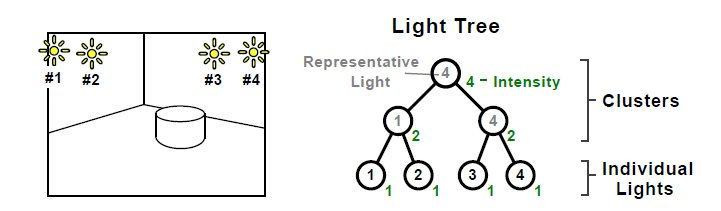
\includegraphics[width=1.0\textwidth]{lightTree.jpg}
  \caption{Example of a light tree.}
	\label{fig:lightTree}
\end{figure}

\underline{Matrix Sampling}: Another adaption of the VPL method in offline rendering techniques is with the use of mathematical matrix sampling to reduce the rendering cost.  In \textit{Matrix Row-Column Sampling for the Many-Light Problem} by Hašan, Pellacini, and Bala (2007), it is shown that many point lights can be seen as a large matrix of sample-light interactions.  The final image is then the sum of all of the columns of the matrix.  Therefore, by sampling this matrix and using a small number of the rows and columns, we can approximate the final image at a fraction of the rendering cost.  The matrix used in this technique is comprised of the columns representing all of the surface points to be lit by each light and each row being comprised of all of the lights in the scene.  Then it can often be shown that this matrix is of low rank meaning that the row and/or columns of the matrix can be linearly combined to form a smaller matrix that would approximate the original larger matrix.  Therefore, this method approaches the problem in a similar way as Lightcuts, but instead of using a tree, we use a matrix.  This method is comprised of four primary steps.  First, we sample $r$ randomly selected rows using shadow maps on the GPU.  Shadow maps will be discussed in the next section.  Next, we partition the reduced columns into clusters on the CPU.  Third, we pick a representative from each cluster to be scaled appropriately to account for the entire cluster on the CPU.  Last, we accumulate each of these representatives using shadows maps on the GPU.  By using this method, the render time of shading $m$ surface points using $n$ VPL's is reduced from $O(mn)$ to $O(m+n)$ as seen in figure \ref{fig:matrixSampling} by Hašan et al. (2007).  Additionally, \textit{LightSlice: Matrix Slice Sampling for the Many-Lights Problem} by Ou and Pellacini (2011) uses a similar approach as in Hašan et al. (2007) and Walter et al. (2005), but found that neither technique optimally exploits the structure of the matrices in scenes with large environments and complex lighting so some modifications were made to reduce render time and improved overall quality.

\begin{figure}[h!]
  \centering
    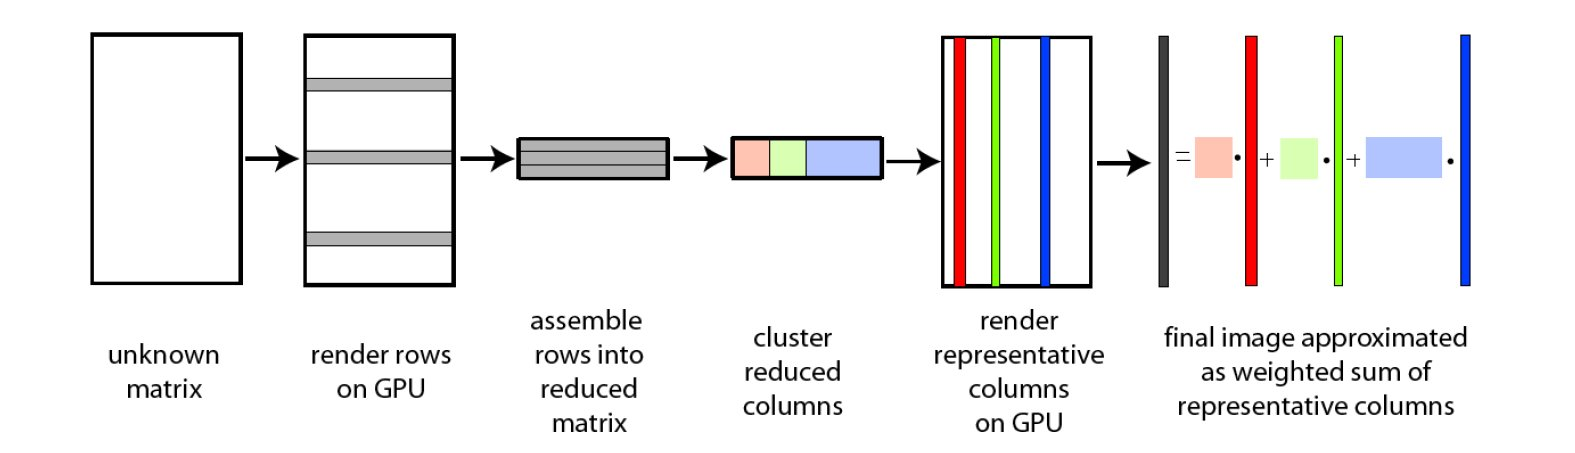
\includegraphics[width=1.0\textwidth]{matrixSampling.jpg}
  \caption{Overview of matrix sampling algorithm.}
	\label{fig:matrixSampling}
\end{figure}
\underline{Shadow Maps}: Shadow maps are textures that are typically used to render shadows, but as shown in the real-time rendering techniques section, they have additional uses.  They are created in a render pass where the view of the scene is computed from the light source's point of view and the distances from the light to the nearest surface for each pixel is stored in this texture or buffer to be used for comparisons when rendering the scene from the camera's point of view to determine whether a surface point is in shadow as presented by Williams (1978) and by Reeves, Salesin, and Cook (1987).  See figures \ref{fig:shadowMap1} and \ref{fig:shadowMap2} by Dachsbacher and Stamminger (2005)for an image of a shadow map and the resulting final image, respectively.  Further discussion on shadow maps will be done in the real-time rendering techniques section as well as in the implementation section.
\begin{figure}[h!]
  \centering
    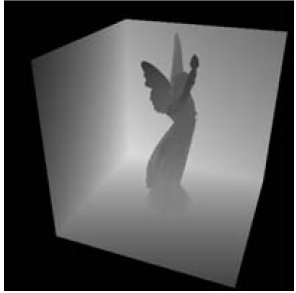
\includegraphics[width=0.5\textwidth]{shadowMap1.jpg}
  \caption{Image of a shadow map. Scene is from the view of the light source.}
	\label{fig:shadowMap1}
\end{figure}
\begin{figure}[h!]
  \centering
    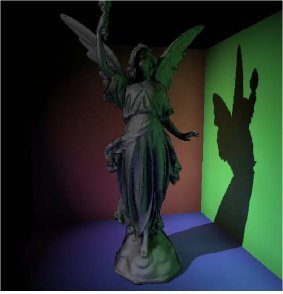
\includegraphics[width=0.5\textwidth]{shadowMap2.jpg}
  \caption{Resulting image using the shadow map from \ref{fig:shadowMap1}.}
	\label{fig:shadowMap2}
\end{figure}
\underline{Virtual Ray Lights}: Lastly, Novák, Nowrouzezahrai, Dachsbacher, and Jarosz (2012) describes a technique to render scenes with single/multiple light scattering in participating media in \textit{Virtual Ray Lights for Rendering Scenes with Participating Media}.  The technique modifies the idea of using VPL's by instead using virtual ray lights or VRL's inside the participating media.  So instead of evaluating each VPL at discrete locations, we calculate the contribution of each VRL with an efficient Monte Carlo sampling technique.  Monte Carlo sampling involves the use of randomly selecting a point based off a probability distribution and is often used for sampling in a wide variety of techniques.  The reason for using VRL's over VPL's is that VPL's can be negatively affected by singularities in the scene.  A singularity is when a given value or location is undefined in our equation.  For example, the equation $1/x$ is undefined for $x=0$.  Singularities are common along boundaries of walls as seen in figure \ref{fig:singularity} by Dachsbacher and Stamminger (2005).  These singularities can cause artifacts in the scene such as spikes of high intensity which can be eliminated through the use of clamping or blurring.  But by using a VRL, we compute the contribution of the light by distributing the energy over a line segment reducing singularities as shown in figure \ref{fig:vrl} by Novák et al. (2012).  In this case, instead of having spikes of high intensity, we have a uniform noise distributed evenly over the image which would be more pleasing to the eye.

\begin{figure}[h!]
  \centering
    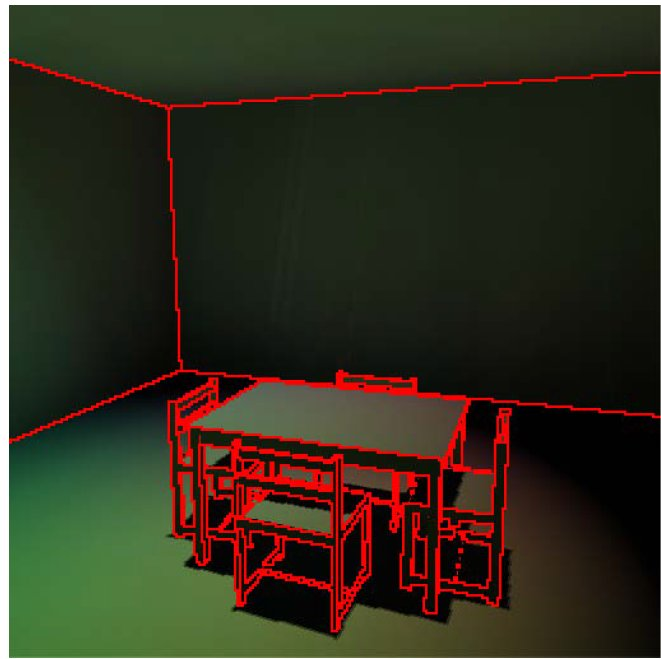
\includegraphics[width=0.5\textwidth]{singularity.jpg}
  \caption{Common locations where singularities exist.}
	\label{fig:singularity}
\end{figure}

\begin{figure}[h!]
  \centering
    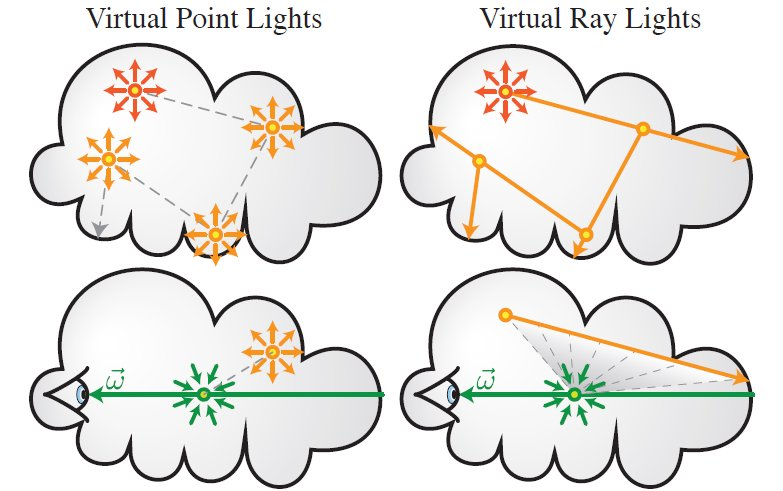
\includegraphics[width=1.0\textwidth]{vrl.jpg}
  \caption{VRL versus VPL.}
	\label{fig:vrl}
\end{figure}

\section{Real-Time Rendering Techniques} \label{sec:RT}
\paragraph{}
With the advancement of technology and the expanded use of the GPU, many offline rendering techniques have been adapted to work on the GPU to run in real-time usually by making trade offs and approximations.  This includes interactive ray tracing by Wald, Kollig, Benthin, Keller, and Slusallek (2002), approximate ray tracing on the GPU by Szirmay-Kalos, Aszodi, Lazanyi, and Premecz (2005), image space photon mapping by McGuire and Luebke (2009), and \textit{Instant Radiosity} by Keller (1997).  The most significant advancement coming from the idea of virtual point lights as in \textit{Instant Radiosity}.

\subsection{\textit{Instant Radiosity}} \label{sec:instantradiosity}
\paragraph{}
As discussed in prior sections, \textit{Instant Radiosity} introduces the technique of approximating indirect illumination by using virtual points lights where each individual light acts independently as a producer of indirect illumination and behaves like a normal point light source.  In the original technique, these VPL's are generated using a quasi-random walk technique created at the hit points of the photons as they are traced into the scene from the primary light source seen in figure \ref{fig:vrl}.  The contributions of these VPL's are then summed through the use of multiple rendering passes.  This implementation had a few limitations such as requiring many rendering passes to support dynamic objects or lights as well as being limited to simple environments due to the high cost of computing shadows for each of the VPL's.  These shadows had to be computed by using shadow volumes or shadow maps and were the bottleneck of the technique.  There were also issues with low sampling rates which would result in weak singularities when the VPL got increasingly close to the illuminated surface point and each VPL had a high influence or contribution on the overall color of the final image.  Also, temporal flickering could be seen if there were not enough VPL's being used.  Despite these issues, real-time performance was attainable in 1997 through the use of this technique.

\subsection{Adaptations of \textit{Instant Radiosity}}
\paragraph{}
In addition to the offline techniques already mentioned which adapted the idea of using VPL's for the offline rendering of a variety of lighting phenomena, many real-time techniques also adapted the use of VPL's.

\underline{Shadow Map Alterations}: As teased in section \ref{sec:otheroffline}, many real-time rendering techniques expanded the use of shadow maps beyond just creating shadows.  \textit{Translucent Shadow Maps} by Dachsbacher and Stamminger (2003) extended the binary shadow map look-up to a shadow map filter to assist in the implementation of real-time sub-surface scattering.  Translucent Shadow Maps extend shadow maps by having additional information stored such as depth and incident light information.  Therefore, each pixel in the Translucent Shadow Map stores the 3D position of the surface sample, the irradiance entering the object at that sample, and the surface normal.  Although this implementation was for sub-surface scattering, it would lead to a development in rendering indirect illumination as well.

\paragraph{}
From this idea of extending shadow maps came further developments in \textit{Reflective Shadow Maps} abbreviated RSM by Dachsbacher and Stamminger (2005).  This technique extended a shadow map such that each pixel in the shadow map would be thought of as an indirect light source.  The reflective shadow map then stored information such as depth value, world space position, normal, and reflected radiant flux shown in figure \ref{fig:RSM} by Dachsbacher and Stamminger (2005).  With all this information available, we can then approximately calculate the indirect irradiance at a surface point by summing the illumination due to all pixel lights as seen in equations \ref{eqn:RSM1} and \ref{eqn:RSM2}.
\begin{equation}
E_{p} (x,n) = \Phi_{p} {max(0, n_{p} \cdot (x-x_{p})) max(0, n_{p} \cdot (x_{p} - x))  } \div {\| x-x_{p} \|^{4} } \label{eqn:RSM1}
\end{equation}
\begin{equation}
E(x,n) = \sum_{pixels p} E_{p}(x,n) \label{eqn:RSM2}
\end{equation}

\begin{figure}
		\centering
        \begin{subfigure}[b]{0.4\textwidth}
                \centering
                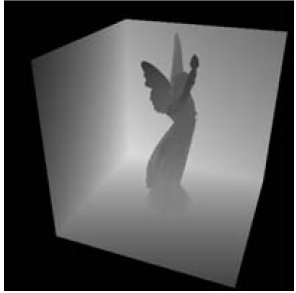
\includegraphics[width=\textwidth]{shadowMap1.jpg}
                \caption{Depth Values.}
                \label{fig:RSM0}
        \end{subfigure}
        \begin{subfigure}[b]{0.4\textwidth}
				\centering
                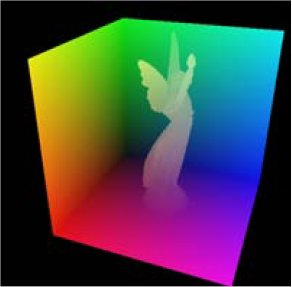
\includegraphics[width=\textwidth]{RSM1.jpg}
                \caption{World Space Positions.}
                \label{fig:RSM1}
        \end{subfigure}
        \begin{subfigure}[b]{0.4\textwidth}
        		\centering
                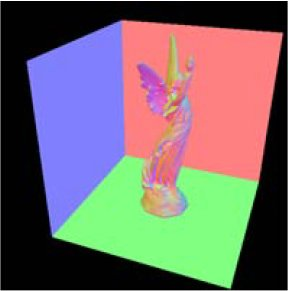
\includegraphics[width=\textwidth]{RSM2.jpg}
                \caption{Normal Values.}
                \label{fig:RSM2}
        \end{subfigure}
        \begin{subfigure}[b]{0.4\textwidth}
        		\centering
                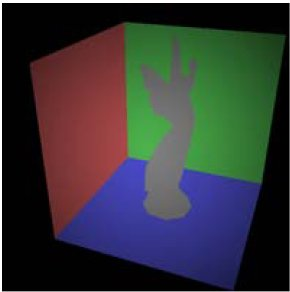
\includegraphics[width=\textwidth]{RSM3.jpg}
                \caption{Reflected Radiant Flux.}
                \label{fig:RSM3}
        \end{subfigure}
        \caption{Data stored in the RSM.}\label{fig:RSM}
\end{figure}

where $x$ is the surface point, $n$ is the normal at $x$, $n_{p}$ and $x_{p}$ is the pixel light normal and position, and $\Phi_{p}$ is the reflected radiant flux of the visible surface point as shown in figure \ref{fig:RSMcalc} by Dachsbacher and Stamminger (2005).  This technique had the same singularity issue near the boundary of two adjoining walls shown earlier in figure \ref{fig:singularity}.  Other limitations includes having to ignore occlusion and visibility for the indirect light sources as well as having to restrict the number of VPL's to around 400 meaning that sampling had to be done to chose the 400 best VPL's.  Also, screen-space interpolation had to be performed by computing the indirect illumination using a low-resolution shadow map and interpolating using multiple low-res samples.  With these restrictions in play, this technique renders approximate indirect illumination for dynamic scenes.

\begin{figure}[h!]
  \centering
    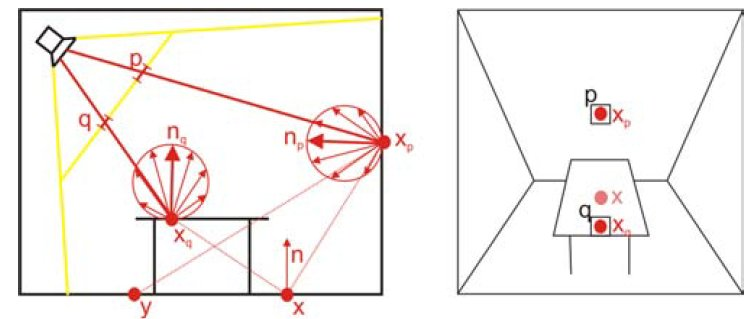
\includegraphics[width=1.0\textwidth]{RSMcalc.jpg}
  \caption{Illustration of equations \ref{eqn:RSM1} and \ref{eqn:RSM2}.}
	\label{fig:RSMcalc}
\end{figure}

\paragraph{}
Reflective shadow maps were then used in many other real-time rendering techniques that followed.  This included \textit{Splatting Indirect Illumination} by Dachsbacher and Stamminger (2006) which rendered the VPL's contributions through a splatting technique in a deferred shading process which reduced the effect of scene complexity on the rendering time.  It also allowed for efficient rendering of caustics and reduced scene artifacts.

\paragraph{}
Additionally, RSM's are used in other applications such as indirect illumination for area light sources as in \textit{Direct Illumination from Dynamic Area Lights With Visibility} by Nichols, Penmatsa, and Wyman (2010).  Here we use RSM's to generate VPL's, but add visibility to the technique by computing occlusion by marching rays towards each VPL through a voxel buffer.  The technique then checks the visibility for each VPL and adds in its illumination provided the VPL is visible.

\paragraph{}
\textit{Imperfect Shadow Maps for Efficient Computation of Indirect Illumination} by Ritschel et al. (2008) altered shadow maps for their purposes by making them imperfect shadow maps or ISM's.  These ISM's were low resolution shadow maps with a simplified point-representation of the scene such that some of the depth values could be incorrect.  This simplified scene is done by approximating the 3D scene by a set of points with a near uniform density which is then used to create an ISM.  The point-based representation of the geometry is used to allow the creation of hundreds of ISM's in parallel in a single pass to support dynamic scenes.  These hundreds of ISM's are stored in a single large texture and are used for approximate visibility for the hundreds or thousands of VPL's used for indirect illumination.  These VPL's are generated through the use of RSM's.  ISM's can also be built on top of reflective shadow maps to create imperfect reflective shadow maps to allow for multiple bounces of light.  With the use of ISM's, indirect illumination scales well with an increase in scene complexity, however, it has no effect on the increase of rendering costs for the direct illumination component.  Limitations include the traditional VPL method issues as discussed in section \ref{sec:instantradiosity}.  Also, indirect shadows cannot be generated for smaller geometry.  Although, this technique calls for inaccurate visibility, it is an upgrade to the strategy of ignoring visibility as in RSM's and it results in a very minimal impact on the final scene but allows for good performance with real-time global illumination shown in figure \ref{fig:ISMcompare} by Ritschel et al. (2008).

\begin{figure}[h!]
  \centering
    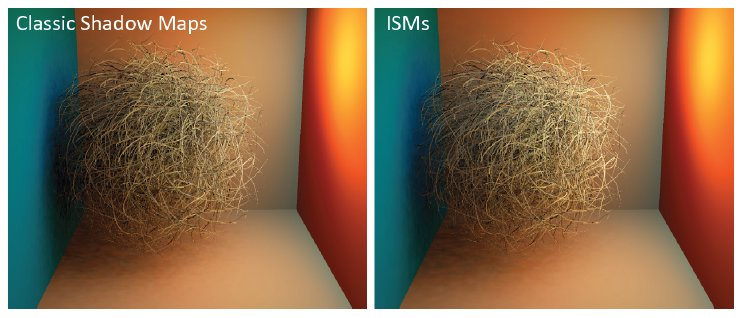
\includegraphics[width=1.0\textwidth]{ISMcompare.jpg}
  \caption{Comparison of normal shadow maps and ISM's.}
	\label{fig:ISMcompare}
\end{figure}

\underline{Screen Space Algorithms}: Additional VPL variants include \textit{Hierarchical Image-Space Radiosity for Interactive Global Illumination} by Nichols, Shopf, and Wyman (2009) where instant radiosity is combined with multiresolution techniques by Nichols and Wyman (2009).  This is done by accumulating indirect illumination at a variety of different resolutions in image space depending upon singularities.  When no singularities are nearby, a lower resolution can be used whereas when there are singularities, a higher resolution should be used to avoid artifacts.  Similar to many of the previous methods mentioned, this techniques ignores visibility for indirect light.

\paragraph{}
Lastly, VPL approaches can introduce bias.  When a VPL is close to a surface, it will introduce a singularity that appears as a high intensity peak in the image.  Most techniques solve this by clamping a VPL's contribution to a surface if it is nearby, however, this removes energy from the system and therefore introduces a bias.  This bias results in darkening of the image near singularity areas such as wall boundaries and edges of objects.  In order to prevent this, screen-space bias compensation by Novák, Engelhardt, and Dachsbacher (2011) was introduced as a post-processing step to recover the clamped energy.  This step involves applying a residual operator to the direct illumination and clamped indirect illumination as computed through the use of the rendering equation (equation \ref{eqn:render}) and a new residual operator.

\subsection{Spherical Harmonics and Lattice-Based Methods}
\paragraph{}
Spherical harmonics are the angular portion of a set of solutions to Laplace's equation represented in a system of spherical coordinates.  Nijasure, Pattanaik, and Goel (2005) used them as a way to represent the incident light at each sample point on a regular grid comprised of both direct and indirect light that arrives from all surface points visible to that sample point in a compact way.  This compact representation is comprised of a small number of coefficients that are computed through the use of a spherical harmonics transformation.  The incident radiance is approximated through the use of a cube map at each grid point, stored as spherical harmonics coefficients, and then the indirect illumination is calculated by interpolating the radiance at the nearest grid points.  This techniques allows for indirect occlusion through the use of shadow cube maps, but is expensive for complicated dynamic scenes.  Papaioannou (2011) combined the grid-based radiance caching of Nijasure et al. (2005) and the use of spherical harmonics along with the reflective shadow maps discussed earlier.  Instead of using cube maps to sample the visibility, this technique sampled the RSM to increase performance.  Kaplanyan and Dachsbacher (2010) used a volume-based method with lattices and spherical harmonics to represent the spatial and angular distribution of light in the scene where VPL's from a RSM are inserted into a volume texture.  This light propagation volume allows for iterative propagation of energy among voxels as well as accounting for fuzzy occlusion by storing depth information and RSM's in a separate occlusion volume to compute indirect shadows that are limited to surfaces larger than the grid size.  These light propagation volumes allow for the use of many more VPL's than other methods due to not calculating the contribution of each of the VPL's individually.  The occlusion calculations are also view-dependent which leads to problems such as popping artifacts.